\documentclass[20pt,landscape]{foils}
\usepackage{mbtslides}
\usepackage[english]{babel}
\usepackage{graphicx}
\usepackage{marvosym}
\usepackage{amssymb}% provides \gtrsim
\usepackage{ellipse}
\usepackage{fancyvrb}
\usepackage{ulem}% provides \sout
\usepackage[cm]{sfmath}

\newif\ifrubric
\rubrictrue

%This is supposed to make underscores cut'n'pastable
%Not sure what the lmodern package does or whether it's needed for this.
%But it's not working (though apparently it did in nam2023)
%\usepackage[T1]{fontenc}
%\usepackage{lmodern}
%\usepackage{textcomp}
%\DeclareTextSymbolDefault{\textunderscore}{T1}

\setlength{\unitlength}{1cm}


\newcommand{\bhref}[2]{\href{#1}{{\color{blue}#2}}}
\newcommand{\burl}[1]{{\color{blue}\url{#1}}}
\newcommand{\rfc}[1]{\bhref{https://www.rfc-editor.org/rfc/rfc#1}
{RFC\,#1}}

\newcommand{\buttimg}[1]
{\mbox{\vtop{\vskip-2ex\hbox{\includegraphics[height=3ex]{#1}}}}}
\newcommand{\tcicon}[1]{
   \mbox{\vtop{\vskip-2.5ex\hbox{\includegraphics[height=3ex]{#1}}}}}
\newcommand{\buttitem}[1]{\item[{\makebox[0cm][r]{\tcicon{#1}}}]}
\definecolor{darkergreen}{rgb}{0,0.38,0}
\definecolor{purple}{rgb}{0.8,0,0.8}

% Fixes problem with includegraphics images screwing up colours on their
% page in the output PDF.  I have no idea *how* it fixes it mind.
\pdfpageattr {/Group << /S /Transparency /I true /CS /DeviceRGB>>}

% Oh no, this is required on my Ubuntu 22.04 (though not 20.04) installation
% to make the \ellipse commands work.
\makeatletter
\newdimen\@tempdimd
\makeatother

\begin{document}
\sf

\newcommand{\bigword}[1]{
  \vspace*{7cm}
  \begin{center}
    \color{darkblue}
    \scalebox{3}{
      \Huge\bf #1
    }
  \end{center}
  \addtocounter{page}{-1}
}

\ifrubric

\rightfooter{}
\MyLogo{}

\vspace*{3cm}
\hspace*{5cm}
\begin{minipage}{30cm}
\LARGE
\begin{enumerate}
  \item Wins
  \item Issues
  \item Ins and Outs of FITS
  \item AOB
\end{enumerate}
\end{minipage}

\newpage
\bigword{Wins?}
\newpage
\bigword{Issues?}
\newpage

\fi

\MyLogo{\color{grey}
        Mark Taylor, FITS file format,
        Bristol Astro Dev Group,
        17 January 2025}
\rightfooter{\quad{\color{grey}\thepage/\pageref*{lastPage}}}
\setcounter{page}{1}

\vspace*{1.0cm}
\begin{center}
{\color{darkblue}
\framebox{\Huge\bf
  \begin{minipage}{0cm}
  \begin{tabbing}
  Ins and Outs of FITS 
  \end{tabbing}
  \end{minipage}
}}
\\[2.0cm]
{\Large
  Mark Taylor
}
\\[2.0cm]
{\large\color{grey}
  Bristol Astro Dev Group
  \\[2ex]
  2 May 2025
}
\end{center}

\vspace*{1.5cm}
\begin{center}
  \tiny
  \color{brown}
  \input gitid
\end{center}

\slide{Outline}

\begin{list1}
  \item History
  \item Pros and cons
  \item Format details
  \item Useful tools
\end{list1}

% \slide{Why am I talking about FITS?}
% 
% \begin{list1}
%   \item Hattie had a problem with a FITS file that was quite easy to fix
%   \begin{list2big}
%     \item[] ... if you know a little bit about the format
%   \end{list2big}
%   \item Fergus suggested it
%   \item You will have to use FITS files
%   \item It's a good format for a lot of things,
%         useful to know its pros and cons
% \end{list1}


\slide{Flexible Image Transport System}

\begin{list0}
  \item History:
  \begin{list2big}
    \item Roots in the late 1970s
    \begin{list3}
      \item Work at NRAO, Kitt Peak, Westerbork
    \end{list3}
    \item 1981: First published proposal
          \bhref{https://ui.adsabs.harvard.edu/abs/1981A&AS...44..363W}
                {Wells, Greisen and Harten, A{\&}A {\sl 44}, p.363 (1981)}
    \begin{list3}
      \item {\sl
             ``adoption of a unique interchange tape format to be used for
               transferring digital imagery between cooperating institutions''}
      \item Integer data only (but with provision for real scaling)
    \end{list3}
    \item 1982: Endorsed by IAU
    \item FITS standard versions:
    \begin{list3}
       \item[1993] v1.0 --- IEEE754 floating point values, ASCII table extension
       \item[1998] v1.2 --- IMAGE and BINTABLE extensions
       \item[2005] v2.1b --- 64-bit integers
       \item[2008] v3.0 --- WCS (celestial and spectral)
                   \bhref{https://doi.org/10.1051/0004-6361/201015362}
                         {Pence et al., A\&A {\sl 524}, A42 (2010)}
       \item[2018] v4.0 --- compression, long string keywords, WCS (time)
    \end{list3}
  \end{list2big}
  \item NASA FITS Support Office:
  \begin{list2big}
    \item[] \burl{https://fits.gsfc.nasa.gov/}
            \hspace*{2em}
            {\color{darkgrey} $\longleftarrow$ for all your FITS needs}
  \end{list2big}
\end{list0}

\slide{Pros and Cons}
\vspace*{-0.5cm}

\begin{list1}
  \item Standard, widely used, lots of software
\vspace*{-0.2cm}
  \begin{list2}
    \item Envied by other disciplines who lack standard formats
\vspace*{-0.1cm}
  \end{list2}
  \item Format definition is published, well-defined, readable
        (not defined by software)
  \item Stable.  Conservative.  Changes very slowly.
\vspace*{-0.2cm}
  \begin{list2}
    \item {\sl ``Once FITS forever FITS''}.
          FITS files not versioned.
\vspace*{-0.1cm}
  \end{list2}
  \item Data and metadata simple to read and write
\vspace*{-0.2cm}
  \begin{list2}
    \item By design --- initial implementations were in FORTRAN
\vspace*{-0.1cm}
    \item Data model very limited
\vspace*{-0.1cm}
    \item Metadata model primitive and flat, no namespacing, ASCII-only
\vspace*{-0.1cm}
  \end{list2}
  \item World Coordinate System metadata included
\vspace*{-0.2cm}
  \begin{list2}
    \item Fairly capable (sky, time, spectra) but inflexible
\vspace*{-0.1cm}
  \end{list2}
  \item Predictable layout of image and table data
\vspace*{-0.2cm}
  \begin{list2}
    \item Good for memory mapping and random access
\vspace*{-0.1cm}
  \end{list2}
  \item Some content restrictions
\vspace*{-0.2cm}
  \begin{list2}
    \item $\le$999 table columns (and $\le$999 image dimensions)
\vspace*{-0.1cm}
    \item Not possible to stream table data (row count required up front)
\vspace*{-0.1cm}
    \item Not optimised for parallel I/O
\vspace*{-0.1cm}
  \end{list2}
\end{list1}

\slide{Love it or hate it?}

\begin{picture}(30,0)
  \put(24,-8){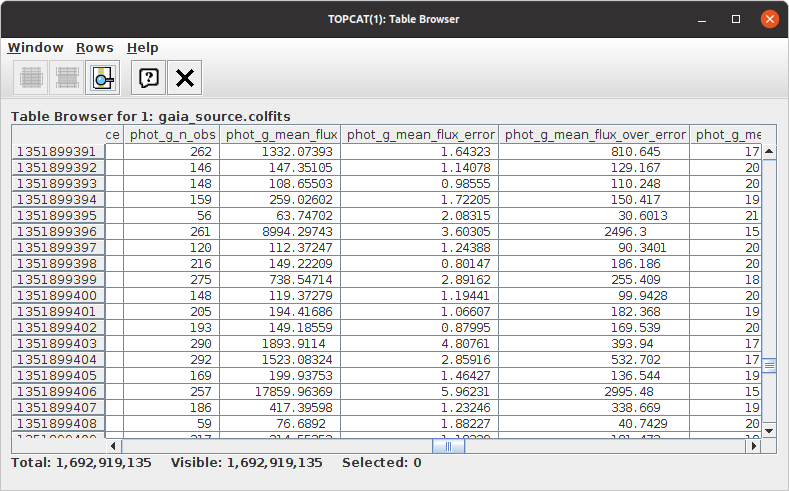
\includegraphics[scale=0.45]{JTable-gaia_source.png}}
  \put(22,-10){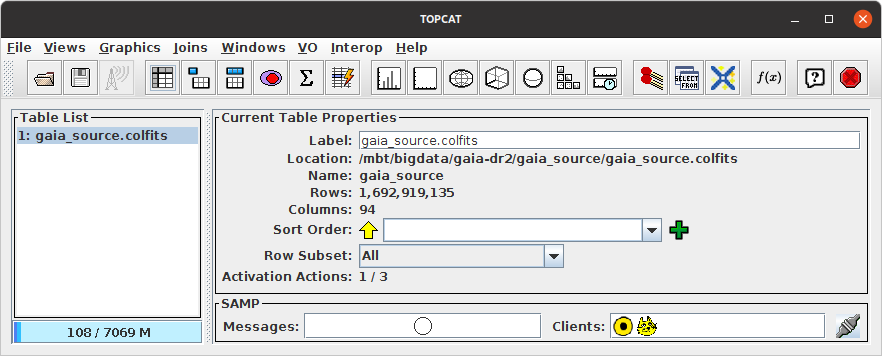
\includegraphics[scale=0.45]{topcat-gaia_source.png}}
\end{picture}
\vspace*{-1.5cm}

\begin{list1}
  \item I like it
  \begin{list2big}
    \item Great for memory-mapped data access in TOPCAT/STILTS
    \item Easy to write a performant I/O library
  \end{list2big}
  \item The Pope likes (liked) it
  \begin{list2big}
    \item In 2010 the Vatican library 
          \bhref{https://www.vaticanlibrary.va/en/the-collections/in-digitalizzation.html}
                {announced decision} \\
          to digitise 80k documents using FITS
  \end{list2big}
  \item The astronomy community is ambivalent
  \begin{list2big}
    \item Papers published bemoaning FITS limitations,
          \\ e.g.\
          \bhref{https://ui.adsabs.harvard.edu/abs/2015A&C....12..133T}
                {Thomas et al., A\&C {\sl 12}, p.133 (2015)}
    \item There are frequent attempts to move \\
          to more modern/capable formats \\
          (HDF5, ASDF, VOTable, Parquet, ...)
    \item But FITS keeps not dying
  \end{list2big}
\end{list1}

\slide{Format Overview}

\begin{picture}(30,0)
  \put(23,-15){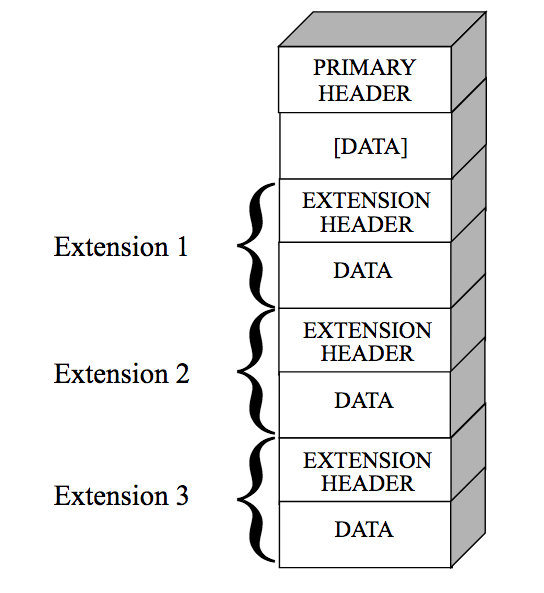
\includegraphics[height=15cm]{fig31_fitsformat.png}}
  \put(32,-16){{\small Credit: \bhref{https://hst-docs.stsci.edu/hstdhb/3-hst-file-formats/3-2-fits-file-format}{STScI}}}
\end{picture}
\vspace*{-1.5cm}

\begin{list0}
  \item Organisation of a FITS file:
  \begin{list2}
    \item Sequence of Header $+$ Data Units (HDUs)
\vspace*{-0.2cm}
    \begin{list3}
      \item Exactly one Primary HDU (PHDU)
      \begin{list4}
\vspace*{-0.2cm}
        \item Data (if present) must be image-like
\vspace*{-0.2cm}
      \end{list4}
      \item Zero or more Extension HDUs
      \begin{list4}
\vspace*{-0.2cm}
        \item Data (if present) may be image- or table-like
              (or, rarely, other things)
\vspace*{-0.2cm}
      \end{list4}
      \item Only way to know how many HDUs is to keep reading
    \end{list3}
\vspace*{-0.2cm}
    \item Each HDU has a Header part and, optionally, a Data part
\vspace*{-0.2cm}
    \item Image data is an N-dimensional array of a single primitive data type
\vspace*{-0.2cm}
    \item Table data is a sequence of rows of typed columns 
\vspace*{-0.2cm}
    \begin{list3}
      \item Each column type is a primitive or N-dimensional array of primitives
    \end{list3}
\vspace*{-0.2cm}
    \item Primitive data types are big-endian 8/16/32/64-bit ints,
                                              32/64-bit IEEE754 floats
    \begin{list3}
      \item No strings as such, but you can use arrays of bytes (ASCII)
    \end{list3}
\vspace*{-0.2cm}
    \item Arrays are column-major (like FORTRAN, not like C/Python)
\vspace*{-0.2cm}
    \item File consists of 2880-byte blocks
\vspace*{-0.2cm}
    \begin{list3}
      \item Header and Data parts aligned on block boundaries, must pad to end
      \item File length is \underline{always} a multiple of 2880
            \hspace*{1em} {\color{darkred}\sl $\longleftarrow$ useful fact!}
      \item[] \hspace*{1.5em}
              \begin{minipage}{25cm}
                {\sl\small\color{darkgrey}
                ``All records will have a length of 23040 bits
                  (2880 8-bit bytes, 3840 6-bit bytes).\\
                  This length is evenly divisible by both the byte and word
                  lengths of all computers \\
                  that have been sold in the commercial market
                  (i.e., 6, 8, 12, 16, 18, 24, 32, \\
                  36, 48, 60 and 64 bits)''}
              \end{minipage}
    \end{list3}
  \end{list2}
\end{list0}

\slide{Header Format}

\begin{list0}
\vspace*{-0.15cm}
  \item Header is a sequence of 80-character ``cards''
\vspace*{-0.15cm}
  \begin{list2big}
    \item Mostly {\color{brown}\tt KEY = value}
    \begin{list3}
      \item Fixed format:
            {\color{brown}\verb*|KEY      = value... / comment...|}
      \item Max keyword length: 8 characters,
            {\color{brown}\verb|[A-Z0-9_-]|}
      \item Value is 7-bit ASCII string, integer, float, complex or boolean
      \item Max value length for string: 68 characters
            (though FITS 4.0 has long strings using {\color{brown}\tt CONTINUE})
      \item Trailing spaces in keyword and string values not significant
\vspace*{-0.15cm}
    \end{list3}
\vspace*{-0.15cm}
    \item Some other miscellaneous card types:
\vspace*{-0.15cm}
    \begin{list3}
      \item {\color{brown}\tt COMMENT},
            {\color{brown}\tt HISTORY},
            {\color{brown}\tt CONTINUE},
            {\color{brown}\tt END},
            blank record
\vspace*{-0.15cm}
    \end{list3}
\vspace*{-0.15cm}
    \item Some keywords defined by FITS standard
\vspace*{-0.1cm}
    \begin{list3}
      \item Mandatory: define layout of data unit
      \begin{list4}
        \item[] {\color{brown}\tt SIMPLE},
                {\color{brown}\tt EXTENSION},
                {\color{brown}\tt BITPIX},
                {\color{brown}\tt NAXIS},
                {\color{brown}\tt PCOUNT},
                ...
\vspace*{-0.15cm}
      \end{list4}
      \item Reserved: useful items to describe data and metadata, incl.\ WCS
      \begin{list4}
        \item[] {\color{brown}\tt DATE},
                {\color{brown}\tt BSCALE},
                {\color{brown}\tt BUNIT},
                {\color{brown}\tt DATAMAX},
                {\color{brown}\tt TELESCOP},
                {\color{brown}\tt TTYPEn},
                {\color{brown}\tt WCSAXESa}, ...
\vspace*{-0.15cm}
      \end{list4}
      \item Otherwise: add any headers you want! (subject to syntax)
      \begin{list4}
        \item Write down somewhere what they mean ... or don't ...
        \item There is a
              \bhref{https://fits.gsfc.nasa.gov/fits_conventions.html}
                    {Registry of FITS conventions}
\vspace*{-0.15cm}
      \end{list4}
\vspace*{-0.15cm}
    \end{list3}
\vspace*{-0.15cm}
    \item Last record must be ``{\color{brown}\tt END}''
\vspace*{-0.15cm}
    \item Pad with spaces to end of 2880-character block
\vspace*{-0.15cm}
  \end{list2big}
\end{list0}

\newcommand{\g}{\color{darkgreen}}

\slide{Primary HDU}

\begin{SaveVerbatim}[commandchars=\\\{\}]{phdu}
\g SIMPLE  =                    T / Written by SkyView Fri Jul 26 06:55:13 EDT 2019
\g BITPIX  =                  -32 / 4 byte floating point
\g NAXIS   =                    2 / Two dimensional image
\g NAXIS1  =                  300 / Width of image
\g NAXIS2  =                  300 / Height of image
 CRVAL1  =                56.75 / Reference longitude
 CRVAL2  =   24.117000000000004 / Reference latitude
 RADESYS = 'FK5     '           / Coordinate system
 EQUINOX =               2000.0 / Epoch of the equinox
 CTYPE1  = 'RA---TAN'           / Coordinates -- projection
 CTYPE2  = 'DEC--TAN'           / Coordinates -- projection
 CRPIX1  =                150.5 / X reference pixel
 CRPIX2  =                150.5 / Y reference pixel
 CDELT1  = -0.00047222219999999997 / X scale
 CDELT2  = 0.00047222219999999997 / Y scale
 COMMENT
 COMMENT SkyView Survey metadata
 COMMENT
 COMMENT Provenance:  Data taken by ROE and AAO, CalTech, Compression
 COMMENT              and distribution by Space Telescope Science Institute
 ...
\g END
\end{SaveVerbatim}

\begin{picture}(30,0)
  \put(19,-12){{\color{brown}\tiny\BUseVerbatim{phdu}}}
\end{picture}
\vspace*{-1.5cm}

\begin{list0}
  \item Primary HDU header:
  \begin{list2big}
    \item Must start {\color{brown}\verb*|SIMPLE  =                    T|}
    \item Contains an {\color{brown}\tt NAXIS}-dimensional array
    \item {\color{darkgreen}\tt SIMPLE},
          {\color{darkgreen}\tt BITPIX},
          {\color{darkgreen}\tt NAXIS},
          {\color{darkgreen}\tt NAXISn} \\
          must appear at the start, in that order
    \item {\color{brown}\tt BITPIX} defines array data type
    \begin{list3}
      \item 8, 16, 32, 64 $\rightarrow$ 8, 16, 32, 64-bit integer
      \item -32, -64 $\rightarrow$ 32, 64-bit floating point
    \end{list3}
    \item {\color{brown}\tt NAXIS},
          {\color{brown}\tt NAXISn} define dimensions of data array
    \begin{list3}
      \item[] {\footnotesize
               $N_{bits} = |{\sc BITPIX}| \times 
               ({\sc NAXIS1} \times {\sc NAXIS2} \times ...
                             \times {\sc NAXISm})$}
    \end{list3}
    \item {\color{brown}\tt NAXIS} may be zero for dataless PHDU
  \end{list2big}
\end{list0}

\slide{IMAGE extension HDU}

\begin{SaveVerbatim}[commandchars=\\\{\}]{imghdu}
\g XTENSION= 'IMAGE   '           / IMAGE extension
\g BITPIX  =                   16 / number of bits per data pixel
\g NAXIS   =                    2 / number of data axes
\g NAXIS1  =                 2080 / length of data axis 1
\g NAXIS2  =                 4608 / length of data axis 2
\g PCOUNT  =                    0 / required keyword; must = 0
\g GCOUNT  =                    1 / required keyword; must = 1
 BZERO   =                32768 / offset data range to that of unsigned short
 BSCALE  =                    1 / default scaling factor
 INHERIT =                    F / inherit the primary header
 DATATYPE= 'Intensity'          / Type of Data
 CTYPE1  = 'RA---TAN'           / R.A. in tangent plane projection
 CRPIX1  =     3134.50385556327 / Ref pix of axis 1
 CRVAL1  =     24.1738207380909 / RA at Ref pix in decimal degrees
 CTYPE2  = 'DEC--TAN'           / DEC. in tangent plane projection
 CRPIX2  =      2288.6460190062 / Ref pix of axis 2
 CRVAL2  =     15.7831584515202 / DEC at Ref pix in decimal degrees
 CD1_1   = 1.59032708066515E-05 / WCS matrix element 1 1
 CD1_2   = -1.24467859737424E-05 / WCS matrix element 1 2
 CD2_1   = -1.24395002801856E-05 / WCS matrix element 2 1
 CD2_2   = -1.59256867637214E-05 / WCS matrix element 2 2
 RADECSYS= 'FK5     '           / R.A./DEC. coordinate system reference
 EQUINOX =                2000. / Equinox of coordinate system
 MJD-OBS =     52135.5547471556 / MJD of start of obseration
 CCDNAME = 'EEV 9273-16-03'     / CCD chip name(s)
 AMPNAME = 'EEV 9273-16-03, right' / Amplifier name(s)
 GAIN    =     2.03999996185303 / Amplifier gain
 RDNOISE =                  3.5 / Readout noise
 EXTVER  =                   -1 / Number assigned to a FITS extension.
 ...
\g END
\end{SaveVerbatim}

\begin{picture}(30,0)
  \put(19,-16){{\color{brown}\tiny\BUseVerbatim{imghdu}}}
\end{picture}
\vspace*{-1.5cm}

\begin{list0}
  \item IMAGE extension HDU header:
  \begin{list2big}
    \item Basically the same as Primary HDU
    \begin{list3}
       \item ... but must start {\color{brown}\verb*|XTENSION= 'IMAGE   '|}
       \item and must have {\color{brown}\tt PCOUNT = 0}, 
                           {\color{brown}\tt GCOUNT = 1} as listed
    \end{list3}
  \end{list2big}
\end{list0}

\slide{BINTABLE extension HDU}

\begin{SaveVerbatim}[commandchars=\\\{\}]{tblhdu}
\g XTENSION= 'BINTABLE'           / binary table extension
\g BITPIX  =                    8 / 8-bit bytes
\g NAXIS   =                    2 / 2-dimensional table
\g NAXIS1  =                   36 / width of table in bytes
\g NAXIS2  =                10000 / number of rows in table
\g PCOUNT  =             40960000 / heap size (no gap)
\g GCOUNT  =                    1 / one data group
\g TFIELDS =                    5 / number of columns
 EXTNAME = 'SimulatedSky-10000' / table name
 TTYPE1  = 'source_id'          / label for column 1
\g TFORM1  = 'J       '           / format for column 1
 TNULL1  =          -2147483648 / blank value for column 1
 TTYPE2  = 'ra      '           / label for column 2
\g TFORM2  = 'E       '           / format for column 2
 TUNIT2  = 'deg     '           / units for column 2
 TCOMM2  = 'ICRS Right Ascension'
 TUCD2   = 'pos.eq.ra'          / VO Unified Content Descriptor for column 2
 TTYPE3  = 'dec     '           / label for column 3
\g TFORM3  = 'E       '           / format for column 3
 TUNIT3  = 'deg     '           / units for column 3
 TCOMM3  = 'ICRS Declination'
 TUCD3   = 'pos.eq.dec'         / VO Unified Content Descriptor for column 3
 TTYPE4  = 'name    '           / label for column 4
\g TFORM4  = '12A     '           / format for column 4
 TTYPE5  = 'spectrum'           / label for column 5
\g TFORM5  = 'PJ(1024)'           / format for column 5
 DATE-HDU= '2025-04-30T15:48:39' / Date of HDU creation (UTC)
 STILVERS= '4.3-2   '           / Version of STIL software
 STILCLAS= 'uk.ac.starlink.votable.UnifiedFitsTableWriter' / STIL Author class
\g END
\end{SaveVerbatim}

\begin{picture}(30,0)
  \put(19,-15){{\color{brown}\tiny\BUseVerbatim{tblhdu}}}
\end{picture}
\vspace*{-1.5cm}

\begin{list0}
  \item BINTABLE HDU header:
  \begin{list2big}
    \item Contains tabular data \\
          (fixed number of rows and columns)
    \item Must start {\color{brown}\verb*|XTENSION= 'BINTABLE'|}
    \item Always {\color{brown}\tt BITPIX = 8},
                 {\color{brown}\tt NAXIS = 2},
                 {\color{brown}\tt GCOUNT = 1}
    \item {\color{brown}\tt PCOUNT} gives size of heap for variable-length cells
    \item {\color{brown}\tt TXXXXnnn} describe column {\sl nnn}
    \begin{list3}
      \item Hence maximum column count of 999
    \end{list3}
    \item {\color{brown}\tt TFORMnnn} gives format of column {\sl nnn},
          required
    \begin{list3}
      \item Uses FORTRAN-like format descriptors
    \end{list3}
    \item Other {\color{brown}\tt TXXXXnnn} keywords optional
    \item Row count required in header $\Rightarrow$ can't stream
  \end{list2big}
\end{list0}

\slide{Other HDU Types}

\begin{list1}
  \item ASCII Table extension
  \begin{list2big}
    \item {\color{brown}\verb*|XTENSION= 'TABLE  '|}
    \item Similar functionality to BINTABLE but less flexible and efficient
    \item Human readable (ASCII)
    \item Not often used
  \end{list2big}
  \item Random Groups structure
  \begin{list2big}
    \item Lives inside Primary HDU
    \item Weird and obsolete
  \end{list2big}
  \item Compression
  \begin{list2big}
    \item Images and tables can be stored in compressed blocks in a BINTABLE
          extension
    \item Look for {\color{brown}\tt ZIMAGE}/{\color{brown}\tt ZTABLE = T}
          and a load of other {\color{brown}\tt Z*} keywords
  \end{list2big}
\end{list1}

\slide{Other interesting keywords/conventions}

\begin{SaveVerbatim}[commandchars=\\\{\}]{hierarch}
\rr{HIERARCH} PPAK P1F1 PVERSION = '1.0     ' / PMAS fitsheader version
\rr{HIERARCH} PPAK P1F1 FILENAME = 'run267_00141a.fits' / original filename
\rr{HIERARCH} PPAK P1F1 DATE = '2013-08-10T01:31:59' / file creation
\rr{HIERARCH} PPAK P1F1 OBSERVER = 'Montoya -- Sanchez'
\rr{HIERARCH} PPAK P1F1 OBJECT = 'obj_4_p1_IC 1528'
\rr{HIERARCH} PPAK P1F2 FILENAME = 'run267_00142a.fits' / original filename
\rr{HIERARCH} PPAK P1F2 DATE = '2013-08-10T01:47:46' / file creation
\rr{HIERARCH} PPAK P1F2 OBSERVER = 'Montoya -- Sanchez'
\rr{HIERARCH} PPAK P1F2 OBJECT = 'obj_4_p1_IC 1528'
\rr{HIERARCH} PIPE P1 PIPE OFFX = -3.25 / IFU RA offset from ref coordinate
\rr{HIERARCH} PIPE P1 PIPE OFFY = -3.5 / IFU DEC offset from ref coordinate
\rr{HIERARCH} PIPE P1 PIPE CHISQ = 0.8 / CHISQ of image matching
\rr{HIERARCH} PIPE P1 PIPE PHOTSCL = 0.912 / photometric scale factor
\end{SaveVerbatim}

\newcommand{\rr}[1]{{\color{darkblue}#1}}
\begin{SaveVerbatim}[commandchars=\\\{\}]{continue}
TTYPE12 = 'TimSerCnt'          / TimSerCnt : PHA multiscalar binning; 4 bands
TUNIT12 = 'Count   '
TZERO12 =                32768
TDDES12 = 'D[0~3] & E[0~63] & T[0;1;16] & C[(S[msLimit1]~S[msLimit2]),((S[msLi\rr{&}'
\rr{CONTINUE}  'mit2]+1)~S[msLimit3]),((S[msLimit3]+1)~S[msLimit4]),((S[msLimit4]+1\rr{&}'
\rr{CONTINUE}  ')~S[msLimit5])] '
TPACK12 = '16,64   '
TFORM12 = '64I     '
TDIM12  = '(4,16)  '
1CTYP12 = 'CHANNEL '
1CPIX12 = '(S[msLimit1]~S[msLimit2]),((S[msLimit2]+1)~S[msLimit3]),((S[msLimit\rr{&}'
\rr{CONTINUE}  '3]+1)~S[msLimit4]),((S[msLimit4]+1)~S[msLimit5])'
\end{SaveVerbatim}

\begin{picture}(30,0)
  \put(19,-6.5){{\color{brown}\tiny\BUseVerbatim{continue}}}
  \put(19,-14.5){{\color{brown}\tiny\BUseVerbatim{hierarch}}}
  \put(22,-16.5){
     \begin{minipage}{20cm}
       \color{darkgrey}\sl
       Note: syntactically legal FITS, \\
       even where non-standard semantics
     \end{minipage}
  }
\end{picture}
\vspace*{-1.5cm}

\begin{list1}
  \item Value scaling
  \begin{list2}
    \item {\color{brown}\tt BZERO}/{\color{brown}\tt BSCALE},
          {\color{brown}\tt TZEROn}/{\color{brown}\tt TSCALEn}
  \end{list2}
  \item Blank values
  \begin{list2}
    \item NaN for floating point values in array/column
    \item {\color{brown}\tt NULL}/{\color{brown}\tt TNULLn}
          magic values for integer values in array/column
  \end{list2}
  \item Checksums
  \begin{list2}
    \item {\color{brown}\tt DATASUM} and {\color{brown}\tt CHECKSUM}
  \end{list2}
  \item CONTINUE records
  \begin{list2}
    \item Extends 80-character limit for non-standard keywords
    \item Introduced at FITS 4.0, older software may not understand it
  \end{list2}
  \item HIERARCH convention
  \begin{list2}
    \item Adds namespacing to keywords
    \item ... but reduces space for values
    \item Non-standard FITS, some software may not understand it
  \end{list2}
\end{list1}


\slide{Tools}

\begin{SaveVerbatim}{fitsverify}
% fitsverify skysim10.fits
 
              fitsverify 4.20 (CFITSIO V3.470)              
              --------------------------------              
 
 
File: skysim10.fits

2 Header-Data Units in this file.
 
=================== HDU 1: Primary Array ===================
 
*** Error:   Keyword #5, BITPIX is duplicated or out of order.
 
 6 header keywords
 
 Null data array; NAXIS = 0 
 
=================== HDU 2: BINARY Table ====================
 
 30 header keywords
 
 SimulatedSky-10000  (5 columns x 10000 rows)
 
 Col# Name (Units)       Format
   1 source_id            J         
   2 ra (deg)             E         
   3 dec (deg)            E         
   4 name                 12A       
   5 spectrum             PJ(1024)  
 
++++++++++++++++++++++ Error Summary  ++++++++++++++++++++++
 
 HDU#  Name (version)       Type             Warnings  Errors
 1                          Primary Array    0         1     
 2     SimulatedSky-10000   Binary Table     0         0     
 
**** Verification found 0 warning(s) and 1 error(s). ****
\end{SaveVerbatim}

\begin{picture}(30,0)
  \put(22.8,-16.5){
     \colorbox{black}{
        \scalebox{0.85}{\tiny\color{green}\BUseVerbatim{fitsverify}}}
     }
\end{picture}
\vspace*{-1.5cm}


\begin{list1}
\vspace*{-0.2cm}
  \item View/edit headers
\vspace*{-0.2cm}
  \begin{list2}
\vspace*{-0.1cm}
    \item {\color{brown}\tt cat},
          {\color{brown}\tt more},
          {\color{brown}\tt less}, ...
\vspace*{-0.1cm}
    \item {\color{brown}\tt vim -b} (binary mode), probably other editors
\vspace*{-0.1cm}
    \item[] \hspace*{1em} ... but use an 80-character terminal!
  \end{list2}
\vspace*{-0.2cm}
  \item Validation (check if file is broken)
\vspace*{-0.2cm}
  \begin{list2}
\vspace*{-0.1cm}
    \item {\color{brown}\tt ls -l}, check length is a multiple of 2880
\vspace*{-0.1cm}
    \item {\color{brown}\tt fitsverify} (a.k.a.\ {\color{brown}\tt fverify})
          from FTOOLS
          \hspace*{2em} {\color{darkgrey}$\longrightarrow$}
\vspace*{-0.1cm}
    \item \burl{https://fits.gsfc.nasa.gov/fits_verify.html}
          --- but limit of 40Mb
  \end{list2}
\vspace*{-0.2cm}
  \item General purpose
\vspace*{-0.2cm}
  \begin{list2}
\vspace*{-0.1cm}
    \item {\tt astropy.io.fits}
\vspace*{-0.1cm}
    \item FTOOLS (\burl{https://heasarc.gsfc.nasa.gov/ftools/})
\vspace*{-0.1cm}
    \item CFITSIO C library
  \end{list2}
\vspace*{-0.2cm}
  \item FITS image analysis/manipulation
\vspace*{-0.2cm}
  \begin{list2}
\vspace*{-0.1cm}
    \item SAOImageDS9
\vspace*{-0.1cm}
    \item GIMP
  \end{list2}
\vspace*{-0.2cm}
  \item FITS table analysis/manipulation
\vspace*{-0.2cm}
  \begin{list2}
\vspace*{-0.1cm}
    \item TOPCAT/STILTS
  \end{list2}
\vspace*{-0.2cm}
  \item[] \hspace*{8cm} {\color{darkgrey}\sl ... and many, many more}
\end{list1}

\slide{Summary}

\begin{list1}
  \item Love it or hate it, you will use FITS
  \item It's old and clunky, but still does a good job
  \item It's not that hard to understand and work with
  \item More information: NASA FITS page \ \burl{https://fits.gsfc.nasa.gov/}
\end{list1}

\vspace{6cm}
\begin{center}
  {\color{darkred}\Huge\bf\sl Thanks!}
\end{center}

\label{lastPage}

\ifrubric

\newcommand{\aobSlide}[1]{
\newpage
\rightfooter{}
\MyLogo{}
\begin{picture}(30,0)
  #1
\end{picture}
\bigword{AOB?}
}
\aobSlide{}

\fi

\end{document}

